\documentclass[11pt,a4paper]{article}

% ---------------- Packages ----------------
\usepackage[left=1in,right=1in,top=1in,bottom=1in]{geometry}
\usepackage[T1]{fontenc}
\usepackage{newtxtext,newtxmath}
\usepackage{titlesec}
\usepackage{enumitem}
\usepackage{graphicx}
\usepackage{tabularx}
\usepackage{hyperref}
\usepackage{array}

\hypersetup{
    colorlinks=true,
    urlcolor=blue
}

\setlength{\parindent}{0pt}
\setlist[itemize]{noitemsep, topsep=2pt}

% ---------------- Section Style ----------------
\titleformat{\section}
{\large\bfseries}
{}
{0em}
{}
[\titlerule]

% ---------------- Document ----------------
\begin{document}
\noindent
\begin{minipage}[t]{0.68\textwidth}
    \vspace{0pt}
    \textbf{\LARGE Mehedi Hassan} \\[1mm]
    mehedihassanalif2003@gmail.com \;\textbar\; 01781111990 \\ 
    Mirpur-12, Dhaka 1216
\end{minipage}%
\hfill
\raisebox{-0.5\height}{%
\begin{minipage}[t]{0.28\textwidth}
    \centering
    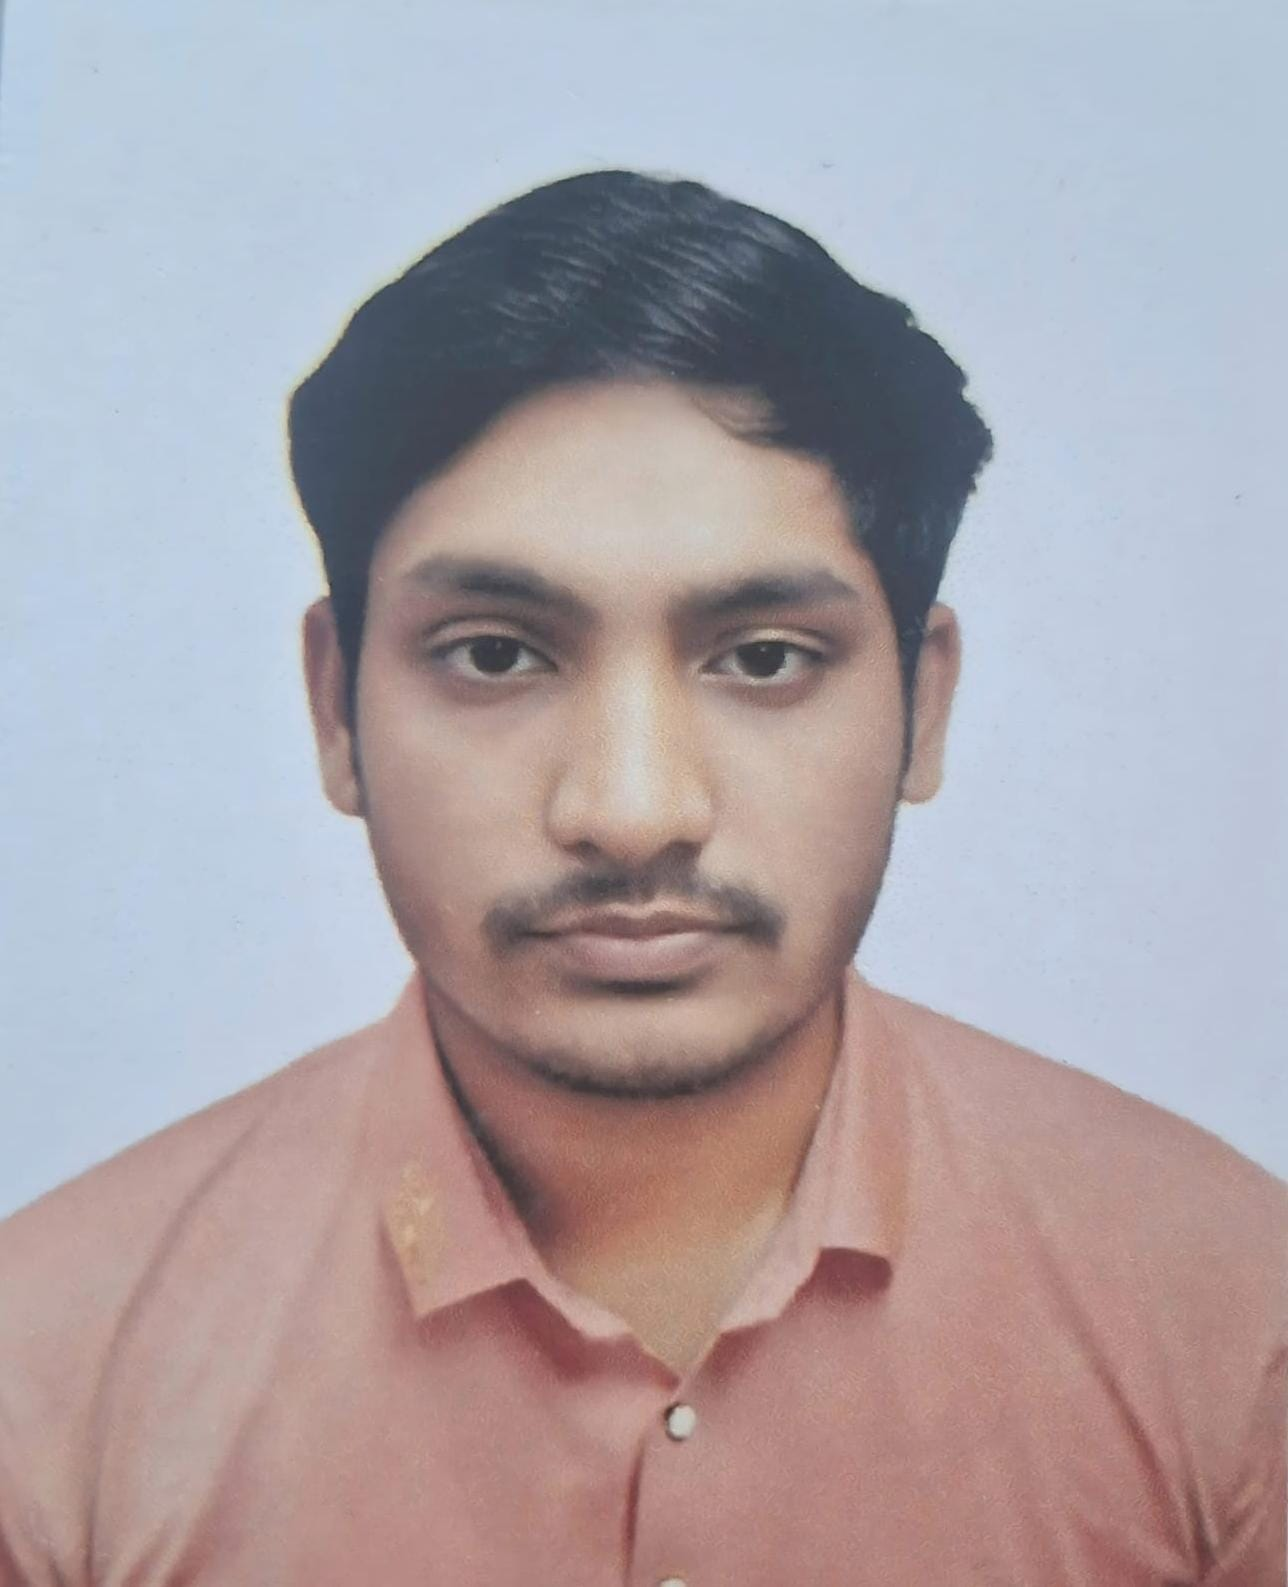
\includegraphics[width=4cm,height=5cm]{pranta_img.jpeg}
\end{minipage}
}

\vspace{10pt}

% ---------------- Career Objective ----------------
\section*{Career Objective}
Motivated and detail-oriented Computer Science and Engineering (CSE) student seeking an entry-level position or internship where I can effectively utilize my computer operation, data entry, and office software skills while gaining practical experience and contributing to organizational growth.

% ---------------- Education ----------------
\section*{Educational Qualification}

\textbf{Bachelor of Science (B.Sc.) in Computer Science \& Engineering (CSE)}\\
Bangladesh University of Business and Technology (BUBT)\\
Result: 3.01 / 4.00 \hfill Passing Year: Continue

\vspace{6pt}

\textbf{Higher Secondary Certificate (HSC)}\\
Adamjee Cantonment College\\
Board: Dhaka, GPA: 5.00 \hfill Passing Year: 2021

\vspace{6pt}

\textbf{Secondary School Certificate (SSC)}\\
Khalishpur M.L. High School\\
Board: Jessore, GPA: 5.00 \hfill Passing Year: 2019

% ---------------- Skills ----------------
\section*{Skills}
\begin{itemize}
    \item Programming Languages: C, C++, Python, JavaScript, Java.
    \item Frontend Technologies: HTML, CSS, JavaScript, React.js, Next.js.
    \item Database: MySQL (Basic), Firebase.
    \item Tools: MS Word, Excel, PowerPoint, VS Code, Kaggle, Google Colab.
    \item Soft Skills: Effective Communication, Leadership, Team Collaboration, Adaptability, Time Management, Creativity.
\end{itemize}

% ---------------- Academic Knowledge ----------------
\section*{Academic Knowledge}
\begin{itemize}
    \item \textbf{Programming and Algorithms:} Programming fundamentals, algorithmic problem solving, data structures (arrays, stacks, queues, linked lists), searching and sorting techniques, and basic complexity analysis.

    \item \textbf{Database Systems:} Database Management Systems (DBMS), relational databases, SQL fundamentals, tables, keys, and relationships.

    \item \textbf{Operating Systems and Networks:} Process management, memory management, CPU scheduling, LAN/WAN, IP addressing, and HTTP/HTTPS basics.

    \item \textbf{Microprocessors and Microcontrollers:} Architecture, instruction sets, interfacing, I/O, and embedded systems.

    \item \textbf{Software Engineering:} Software Development Life Cycle (SDLC), requirements analysis, and basic system documentation.

    \item \textbf{Internet of Things (IoT):} Basics of IoT including sensors, actuators, microcontroller-based systems, and real-time data communication.

    \item \textbf{Cybersecurity:} Common security threats, authentication mechanisms, and basic security principles.

    \item \textbf{Discrete Mathematics:} Basics of logic, sets, relations, and graphs.
\end{itemize}

% ---------------- Projects ----------------
\section*{Projects}
\begin{itemize}[label=\textbullet]
    \item \textbf{Fire-Quake Detection System:} Built an IoT-based system using multiple sensors (MQ2, DHT11, MPU6050) and NodeMCU (ESP8266) to monitor environmental conditions in real time. Implemented alert notifications through the Blynk platform along with local alarms for safety alerts.

    \item \textbf{Women Safety Mobile Application:} Developed a women safety mobile application using React with emergency features such as shake detection, automatic calling, and live location sharing. Enabled quick alerts to predefined contacts during critical situations.
\end{itemize}

% ---------------- Languages ----------------
\section*{Language Proficiency}
\begin{itemize}[label=\textbullet]
    \item \textbf{Bengali:} Mother Tongue
    \item \textbf{English:} Proficient
\end{itemize}

% ---------------- Personal Info ----------------
\section*{Personal Information}
\begin{tabular}{@{}ll@{}}
Father's Name & : Habibur Rahman \\
Mother's Name & : Sheuly Khatun \\
Permanent Address & : Vill: Hat-Khalispur, P.O: Khalishpur, P.S: Moheshpur, Dist: Jhenaidah \\
Present Address & : Road: 20, Block: C, Mirpur 12, Dhaka-1216 \\
Date of Birth & : 26-Aug-2003 \\
Religion & : Islam \\
Marital Status & : Single \\
Blood Group & : O+ \\
Gender & : Male \\
\end{tabular}

% ---------------- Declaration ----------------
\section*{Declaration}
I hereby declare that the information provided above is true and correct to the best of my knowledge and belief.

\vspace{10pt}
\textbf{Signature:} \\[2mm]

\includegraphics[width=3cm]{pranta_sign_img.jpeg}

\end{document}
